\documentclass[14pt]{extarticle}

\usepackage{fontspec}
\setmainfont{Times New Roman}

% размер полей
\usepackage{geometry}
\geometry{a4paper, top=2cm, bottom=2cm, right=1.5cm, left=3cm}

 %debugging
%\usepackage{showframe}

% полуторный интервал
\usepackage{setspace}
\onehalfspacing

% абзацный отступ
\setlength{\parindent}{1.25cm}

% выравнивание текста по ширине
\sloppy

% списки
\usepackage{calc} % арифметические операции с величинами
\usepackage{enumitem}
\setlist{
    nosep,
    leftmargin=0pt,
    itemindent=\parindent + \labelwidth - \labelsep,
}

% подписи к рисункам и таблицам
\usepackage{caption}
\renewcommand{\figurename}{Рисунок}
\renewcommand{\tablename}{Таблица}
\DeclareCaptionFormat{custom}
{
    \textit{#1#2#3}
}
\DeclareCaptionLabelSeparator{custom}{. }
\captionsetup{
    % хз какой это размер - 12 или нет, но выглядит меньше 14
    font=small,
    format=custom,
    labelsep=custom,
}

% картинки
\usepackage{graphicx}

% колонтитулы
\usepackage{fancyhdr}

% картинки и таблицы находятся именно в том месте текста где помещены (атрибут H)
\usepackage{float}

% таблицы
\usepackage{tabularray}

\graphicspath{ {3.2.1/models/} }
\begin{document}
\pagestyle{fancy}
\fancyhead{}
% disable header
\renewcommand{\headrulewidth}{0pt}
\fancyfoot[L]{Дубровских гр 221-361}
\fancyfoot[C]{ЛР 3.2.1}
\fancyfoot[R]{Продажа автотранспорта}
\singlespacing

\newpage
\begin{center}
    Министерство науки и высшего образования Российской Федерации
    Федеральное государственное автономное образовательное учреждение

    высшего образования

    \guillemotleft МОСКОВСКИЙ ПОЛИТЕХНИЧЕСКИЙ УНИВЕРСИТЕТ\guillemotright

    (МОСКОВСКИЙ ПОЛИТЕХ)
\end{center}
\noindent
\bigbreak
\bigbreak
\bigbreak
\bigbreak
\begin{center}
    ЛАБОРАТОРНАЯ РАБОТА 3.2.1

    По курсу Проектирования пользовательских интерфейсов в веб

    \textbf{Разработка визуальной карты (структуры) сайта}
    \bigbreak
    \bigbreak
    \bigbreak
    \bigbreak
    ТЕМА

    \guillemotleft\textbf{САЙТ ДЛЯ ПРОДАЖИ И ПОИСКА АВТОМОБИЛЕЙ}\guillemotright
\end{center}
\noindent
\bigbreak
\bigbreak
\bigbreak
\bigbreak
\bigbreak
\bigbreak
\bigbreak
\bigbreak
\bigbreak
\bigbreak
\hfill Выполнил

\hfill Дубровских Никита Евгеньевич

\hfill Группа 221-361
\bigbreak
\bigbreak
\bigbreak
\hfill Проверил

\hfill Натур ВВ
\vfill
\begin{center}
    Москва, 2024
\end{center}
\newpage
\onehalfspacing


\begin{center}
    \textbf{Лабораторная работа 3.2.1}

    \textbf{Разработка визуальной карты (структуры) сайта}
\end{center}

\textbf{Цель работы:} продумать все необходимые экраны будущего интерфейса сайта и выстроить структуру сайта
\bigskip

\textbf{Задачи:}

\begin{enumerate}
    \item Определить необходимое количество экранов проектируемого интерфейса сайта (не менее 10).
    \item Проанализировать структуру сайтов-аналогов. Построить карту сайта одного из аналогов (есть ресурсы, где встроена эта функция)
    \item Построить обобщенную структурную схему карты сайта с учетом иерархии и логических взаимосвязей экранов.
    \item Добавить на экраны информацию о базовых элементах, находящихся на них (можно добавлять комментарии).
\end{enumerate}
\bigskip

\textbf{Основные термины}

\begin{itemize}
    \item Интерфейс сайта - визуальная и функциональная часть сайта, с которой взаимодействует пользователь.
    \item Структура сайта - организация и иерархия страниц сайта, определяющая, как они связаны друг с другом.
    \item Карта сайта - графическое представление структуры сайта, показывающее взаимосвязи между страницами.
    \item Аналоги - сайты, имеющие схожую тематику или функционал, используемые для анализа и сравнения.
    \item Базовые элементы - основные компоненты интерфейса, такие как кнопки, меню, формы и т.д.
    \item UX (User Experience) - опыт пользователя, связанный с взаимодействием с продуктом или услугой.
    \item Контент - информация, представленная на сайте, включая текст, изображения, видео и другие медиаформаты.
    \item SEO (Search Engine Optimization) - оптимизация сайта для поисковых систем, направленная на повышение его видимости.
    \item Цифровые генераторы карт сайта - инструменты, позволяющие автоматически создавать карты сайта на основе заданных параметров.
\end{itemize}
\bigskip

\textbf{Карта сайта}
\bigskip

На рисунках 1-2 изображена карта сайта аналога drom.ru разбитая на 2 изображения для повышения читабельности.
\bigskip

\noindent
\begin{minipage}{\linewidth}
    \fbox{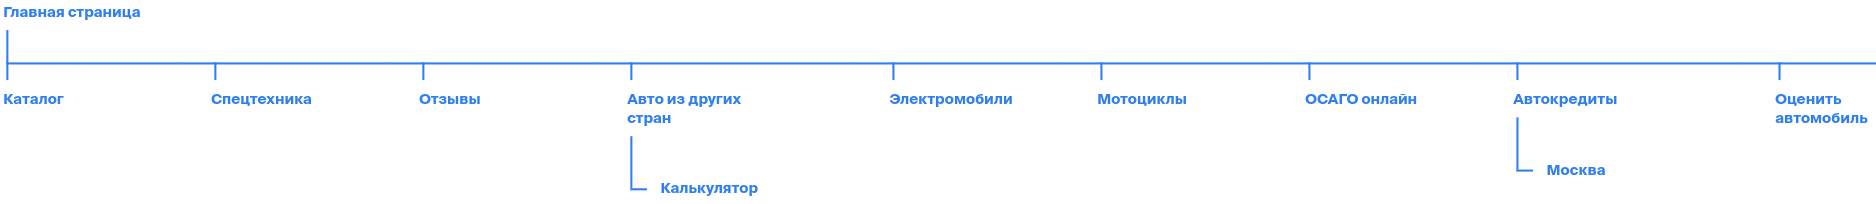
\includegraphics[width=\linewidth]{drom_sitemap1_2}}
    \captionof{figure}{Левая часть карты сайта drom.ru}
\end{minipage}
\bigskip

\noindent
\begin{minipage}{\linewidth}
    \fbox{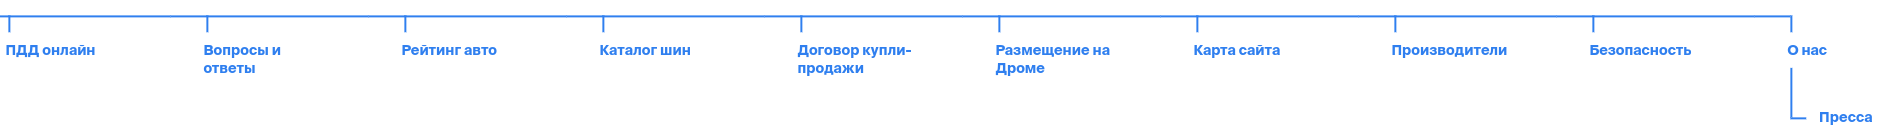
\includegraphics[width=\linewidth]{drom_sitemap2_2}}
    \captionof{figure}{Правая часть карты сайта drom.ru}
\end{minipage}
\bigskip

На рисунке 3 представлена обощенная структурная схема карты сайта с учётом иерархии и логических взаимосвязей экранов. Также была добавлена информация о базовых элементах на страницах.

\noindent
\begin{minipage}{\linewidth}
    \fbox{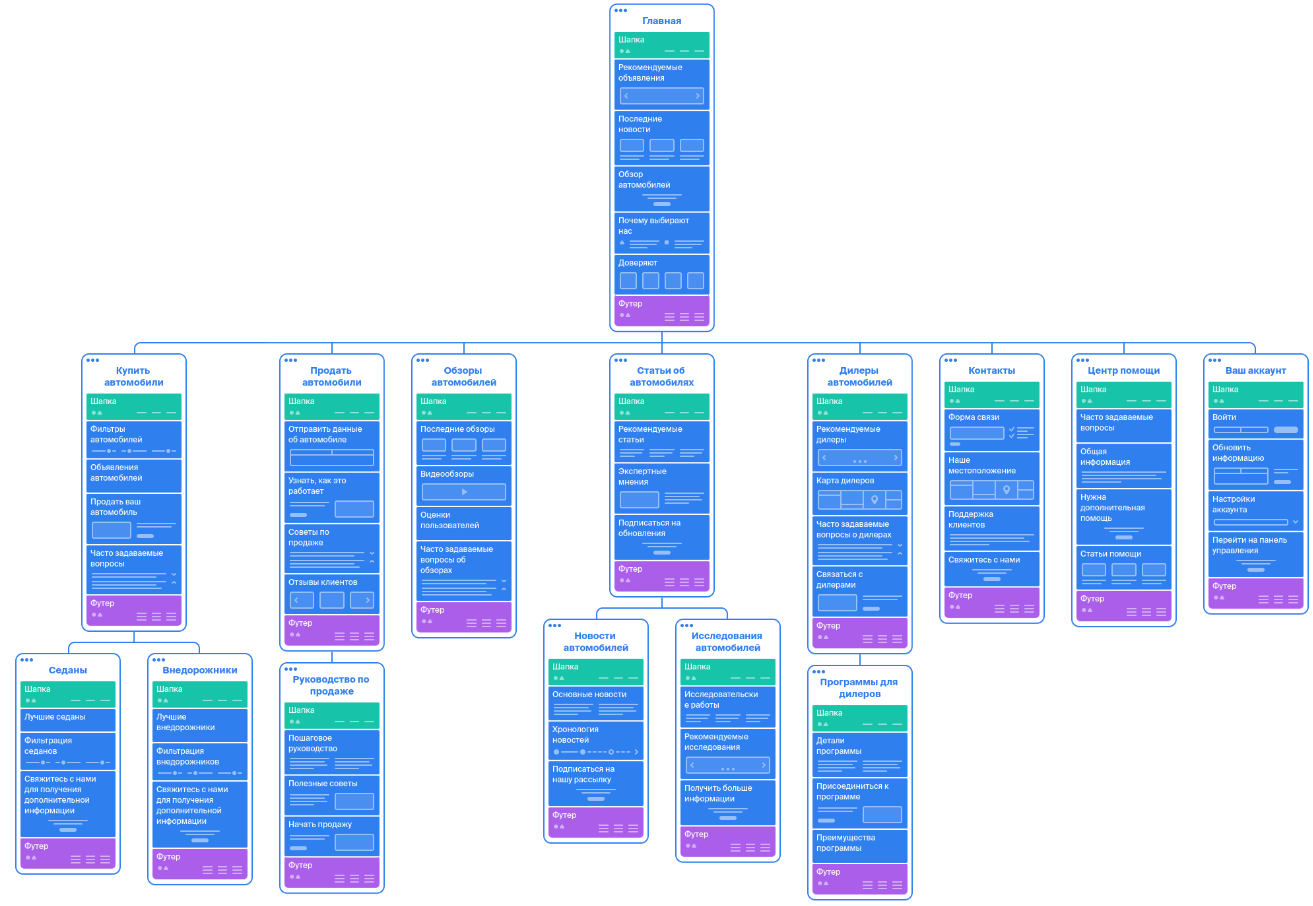
\includegraphics[width=\linewidth]{mysite_sitemap}}
    \captionof{figure}{Обобщённая структурная схема карты сайта}
\end{minipage}
\bigskip

\textbf{Контрольные вопросы и ответы}

\begin{enumerate}
    \item Что такое «визуальная карта сайта»?

Визуальная карта сайта — это графическое представление структуры сайта, которое показывает, как страницы связаны друг с другом. Она отображает иерархию страниц, их взаимосвязи и навигацию, что позволяет лучше понять, как будет организован контент на сайте.
    \item Зачем карта нужна?

Карта сайта необходима для:
        \begin{itemize}
            \item Определения структуры и иерархии страниц.
            \item Упрощения навигации для пользователей.
            \item Помощи в планировании контента и задач для команды.
            \item Обсуждения с клиентом и устранения недопонимания на ранних этапах проектирования.
            \item Оптимизации SEO, так как помогает поисковым системам лучше индексировать сайт.
        \end{itemize}
    \item Какие программы для проектирования карты сайта и процессов вам известны?

        \begin{itemize}
            \item FlowMapp — инструмент для создания визуальных карт сайта и планирования пользовательских потоков.
            \item Octopus.do — визуальный инструмент для генерации карт сайта, позволяющий быстро создавать структуру сайта.
            \item MindMeister — программа для создания ментальных карт, которая может быть использована для проектирования структуры сайта.
            \item Slickplan — инструмент для создания карт сайта и планирования контента.
        \end{itemize}
    \item Расскажите про основные возможности этих программ.

        \begin{itemize}
            \item FlowMapp: создание интерактивных карт сайта, блок-схем, возможность работы в команде, шаблоны для различных типов проектов.
            \item Octopus.do: быстрое создание визуальных карт сайта, возможность анализа сайтов-аналогов, экспорт карт в различные форматы.
            \item MindMeister: создание ментальных карт, возможность совместной работы, интеграция с другими инструментами.
            \item Slickplan: создание карт сайта, генерация диаграмм, возможность добавления контента и заметок к страницам.
        \end{itemize}
    \item Расскажите про известные вам виды структуры сайта.

        \begin{itemize}
            \item Иерархическая структура: страницы организованы в виде дерева, где главные страницы ведут к подстраницам.
            \item Линейная структура: страницы расположены последовательно, одна за другой, что подходит для простых сайтов.
            \item Сеточная структура: страницы связаны между собой в виде сетки, что позволяет пользователю свободно перемещаться между ними.
            \item Смешанная структура: комбинирует элементы различных структур, обеспечивая гибкость навигации.
        \end{itemize}
    \item Как можно использовать «карту сайта» для UX этапа проектирования?

Карта сайта помогает на этапе UX проектирования, так как:
        \begin{itemize}
            \item Позволяет визуализировать навигацию и структуру, что упрощает понимание пользовательского пути.
            \item Помогает выявить потенциальные проблемы с навигацией и доступностью информации.
            \item Способствует более эффективному планированию контента и функционала, основываясь на потребностях пользователей.
            \item Упрощает тестирование и обсуждение дизайна с командой и клиентами, позволяя сосредоточиться на пользовательском опыте.
        \end{itemize}
\end{enumerate}

\end{document}
